%
% Based on the work done for our Iterative Compiler at York
%
%
%I don't think we need this.

%\begin{abstract}
%
%Using static analysis techniques compilers for lazy functional languages can be
%used to identify parts of a program that can be legitimately evaluated in
%parallel and ensure that those expressions are executed concurrently with the
%main thread of execution. These techniques can produce improvements in the
%runtime performance of a program, but are limited by the static analyses' poor
%prediction of runtime performance.  This paper outlines the development of a
%system that uses iterative profile-directed improvement \emph{in addition to}
%well-studied static analysis techniques. This allows us to achieve higher
%performance gains than through static analysis alone.
%
%\end{abstract}
%
%\keywords
%Implicit Parallelism, Lazy Functional Languages, Automatic Parallelism,
%Strictness Analysis, Projections, Iterative Compilation, Feedback Directed Compilation

\section{Introduction}
\label{section:Introduction}

%\epigraph{I thought the ``lazy functional languages are great for implicit 
%parallelism'' thing died out some time ago \citep{benEmail}}{Ben Lippmeier}

Advocates of purely functional programming languages often cite easy
parallelism as a major benefit of abandoning mutable state \citep{hughes:thesis,
SPJ:PIFPL}. This idea drove research into the theory and implementation of
compilers that take advantage of \emph{implicit parallelism} in a functional
program. For lazy functional languages this can be seen to be at odds with the
goal of only evaluating expressions when they are needed. 

The ultimate goal of writing a program in a functional style, and having the
compiler find the implicit parallelism, still requires work.  We believe there
are several reasons why previous work into implicit parallelism has not
achieved the results that researchers have hoped for. Chief amongst those
reasons is that the static placement of parallel annotations is not sufficient
for creating well-performing parallel programs \citep{hammond2000research,
hogen1992automatic, tremblay1995impact, feedbackImplicit}. This paper explores
one route to improvement: the compiler can use runtime profile data to improve
initial decisions about parallelism in much the same way a programmer would
manually tune a parallel program.

Additionally, when research into implicit parallelism was more common, the work
was often based on novel architectures or distributed systems, not commodity
hardware \citep{GRIP, hammond2000research}. Research was unable to keep
up with huge improvements in sequential hardware. Today most common desktop
workstations are parallel machines; this steers
our motivation away from the full utilisation of hardware. Many programmers
today write sequential programs and run them on parallel machines. We
argue that even modest speedups are worthwhile if they occur `for free'.

\begin{figure}
  \input{Informed/SumPhases/SumEuler.hs}
\caption{Source listing for \texttt{SumEuler}}
\label{sumOrig}
\end{figure}

Imagine that we have written the program in Figure \ref{sumOrig}. We might
study its structure and decide to introduce some \verb-par- annotations.  When
the program is compiled and executed, if we find that performance is still not
satisfactory, we might study a profile (e.g. as provided by threadscope
\citep{Jones2009Tuning}), return to the source for the program and adjust the
placement of parallel annotations. This is the approach advocated by
\citep{Jones2009Tuning} and \citep{runciman1994profiling}.  In contrast, many of
the previous attempts at automating parallelism only analyse the program
statically and do not adjust any parallel annotations after runtime data is
gathered. This would be equivalent to a programmer never adjusting annotations
after profiling the program.

By using runtime feedback, we can have the compiler \emph{be generous} when
introducing parallelism into the program. The profiling data will then point to
the places where parallel evaluation under-performs and the compiler will
\emph{disable} the parallelism in these places. 


We have designed and implemented an experimental compiler for implicit
parallelism with profile-driven improvement. The source language of the
compiler is FLite \citep{naylor2010reduceron}, a non-strict functional core
language including ADTs, in addition to integer primitives, type checking,
parametric polymorphism, pattern-matching, and higher-order functions. 

\subsection{Contributions}

The contributions of our work are as follows:

\begin{itemize}
    \item A fresh implementation of Hinze's projection-based strictness analysis \citep{hinze1995projection}
        used to derive evaluation strategies
    \item A scheme for introducing parallelism into a program in conjunction with these
        strategies
    \item Simple rules for evaluating the effectiveness of parallelism
    \item A technique to disable \verb-par- annotations
    \item Search strategies to improve initial \verb-par- placements
\end{itemize}


This paper presents an overview of the design of our compiler and some of the
design decisions that were made.  It also presents the results of experiments
using a range of small benchmark programs.

\subsection{Roadmap}

\S\ref{sec:overview} presents a high-level overview of our approach to implicit
parallelism.  \S\ref{sec:defunct} explains the advantages of performing
defunctionalisation on the source program. \S\ref{sec:strictness} motivates our
use of a projection-based strictness analysis.  \S\ref{sec:proAndStrat}
describes the correspondence between projections and strategies which allows us
to generate parallel strategies based on the projections provided by the
strictness analysis. \S\ref{sec:introPar} describes the initial placement of
\verb-par- annotations in the source program. \S\ref{sec:iterate} introduces
the technique used for utilising the runtime profiling to disable some of the
introduced parallelism along with possible additional search techniques.
\S\ref{sec:results} presents some experimental results and discussion of those
results. Lastly, \S\ref{sec:conclusion} contains our conclusions and thoughts
on possible future work.

\section{Overview}
\label{sec:overview}

In this section we present the overall picture of our technique. Much of the
discussion will center around the code presented in Figure \ref{sumLast}. In
order to understand the code, it is useful to understand the architecture of the
compiler.

\subsection{Compiler Stages}
The compiler is organised into 8 main phases, as follow:

\begin{enumerate}
    \item Parsing
    \item Defunctionalisation
    \item Projection based Strictness Analysis
    \item Generation of strategies
    \item Placement of \verb-par- annotations
    \item $G$-Code Generation
    \item Execution
    \item Feedback and iteration
\end{enumerate}

The parsing of the source language and sequential $G$-Code generation are done
in the standard way and will not be discussed further. The rest of the paper will
discuss the other phases.

\subsection{A Program Before Iteration}

\begin{figure}[t!]
  \input{Informed/SumPhases/SumEulerProcessed.core}
\caption{Core representation of \texttt{SumEuler} after defunctionalisation, demand
         analysis, and the introduction of initial \texttt{par} sites along
         with their associated strategies.(Auto-generated names have been
         replaced for better readability)}
\label{sumLast}
\end{figure}

The code listed in Figure \ref{sumLast} is the resulting core representation
of the program in Figure \ref{sumOrig} after our analysis and transformations.
Specifically, the program has passed through compiler stages 1-5.

Before we dive into the program itself, note the following points:

\begin{itemize}
    \item We only present the functions that have changed as a result of transformation
    \item We have replaced auto-generated names with easier to read names
    \item Functions ending in `S$N$' are derived strategies
    \item Functions with an underscore in the name are the result of defunctionalisation
\end{itemize}

Taking a look at the program we can see several of the core ideas.

\paragraph{Defunctionalisation}
The application of \verb-map- to \verb-euler- has been replaced by a call to
the specialised \verb-map_euler- function.  We no longer have the functions
\verb-map- or \verb-filter- instead we have specialised versions of these
functions (e.g. \verb-map_euler-)

\paragraph{Introduction of parallelism}
Two calls to \verb-par- have been introduced in the \texttt{main} function. Our
work uses the traditional style for the parallel combinator \citep{strategies}

\begin{verbatim}
    par :: a -> b -> b
    par x y = y
\end{verbatim}

The first argument is \emph{sparked} off to be evaluated in parallel and the
function returns the second argument. This style is what allows us to easily
\emph{switch off} a particular \verb-par- which causes that switched off
\verb-par- to act like \verb-flip const-. This is explored further in
\S\ref{sec:switchPar}.

Each application of \verb-par- introduced by our compiler takes the following
form: \verb-par (s x) e- where \verb-(s x)- is the application of derived
strategy \verb-s- to a variable \verb$x$ and \verb$e$ is an expression containing \verb$x$ as a
free variable.  In a \emph{top-level definition} like \verb-main-, \verb$x$ will be a
name introduced by a \verb-let- expression. For \verb-par-s within the
strategies themselves, \verb$x$ will be a name introduced by case analysis.

\paragraph{Demand Analysis and Strategies}

The compiler has introduced a number of strategies into the program. These
strategies are derived based on the results of a demand analysis. A simple
example from the program is the transformed version of \verb-length-. Because
\verb-+- (for non-lazy integers) requires both arguments to be fully evaluated, it is safe to 
evaluate the arguments to \verb-+- in parallel to the execution of its body.
In order to benefit from the parallel evaluation, the structure must be shared.
The introduction of the name \verb-len- accomplishes this. Because the type
of \verb-len- is \verb-Int- evaluating the expression to WHNF is sufficient to
evaluate the value fully. 

Looking at the body of \verb-euler- where \verb-length- is called we see a
similar pattern. In this case the demand analysis determines that it is
safe the evaluate the \emph{spine} of the list passed to \verb-length-.
The expression is given the name \verb-ys- and the strategy \verb-eulerListS1-
is derived based on this information. Notice that the elements of the list
passed to \verb-eulerListS1- are ignored in its body. 

There are cases where there is a strict demand on an expression but we
do not introduce parallel evaluation of the expression. This can be seen
in the first argument to \verb-+- in the body of \verb-length-. The rules
for which subexpressions are considered \emph{definitely} not worthwhile
are discussed in \S\ref{sec:introPar}.

\paragraph{Iterative Improvement}

Just because an expression is \emph{able} to be evaluated in parallel does not
mean that doing so is beneficial! This is one of the critical problems in
implicit parallelism \citep{hogen1992automatic, hammond2000research,
Jones2009Tuning}. To combat this we run the program as presented in Figure
\ref{sumLast} and collect statistics about the amount of productive work
each \verb-par- is responsible for. The \verb-par-s that do not introduce
a worthwhile amount of parallelism (see discussion in \S\ref{sec:iterate})
are disabled, freeing the program from incurring the overhead of managing
threads for tasks with insufficient granularity \footnote{This can be seen
as a more extreme variation of Clack and Peyton Jones' ``Evaluate and die!''
model of parallelism \citep{clack1986four}: Evaluate \emph{a lot} or die!}.

Earlier we mentioned the \verb-par-s in the bodies of \verb-length- and
\verb-euler-. We picked these examples because while they are safe, they are
not likely to be worthwhile. In the body of \verb-length- the parallel
evaluation of \verb-len- only evaluates what \verb-+- will immediately evaluate
anyway. Giving us no benefit from parallelism. The parallel evaluation of
\verb-ys- in the body of \verb-euler- also suffers from a similar issue.

So why introduce this parallelism? Because the granularity and possible
interference of parallel threads is difficult to know \emph{statically} at
compile time. If we err on the side of generosity with our \verb-par-
annotations we can then use \emph{runtime} profiling to gather information
about the granularity and interference of threads. 

As we would hope, our runtime system does determine that these two \verb-par-s (and some
others) are not worthwhile and disables them, improving performance.

\paragraph{}

Now that we have presented the high-level view of our work we can explore each of
the stages in depth and discuss our reasons for certain design decisions.


\section{Defunctionalisation}
\label{sec:defunct}

After parsing the next stage of the compiler applies a defunctionalising
transformation to the input programs. Our defunctionalisation method is limited
in scope, but sufficient for our purposes. It specialises higher-order
functions defining separate instances for different functional arguments. We
are careful to preserve sharing during this transformation. Here we give our
motivation for introducing this transformation.

Central to our design is the concept of \verb-par- placement within a program.
Each \verb-par- application can be identified by its \emph{position} in the
AST. In a higher-order program basing our parallelism on the location of a
\verb-par- would very likely lead to undesirable consequences. For example, a common pattern
in parallel programs is to introduce a parallel version of the \verb-map-
function

\begin{alltt}
    parMap :: (a -> b) -> [a] -> [b]
    parMap f []     = []
    parMap f (x:xs) = let y = f x
                      in y `par` y : parMap f xs
\end{alltt}

There is inevitably some overhead associated with evaluation of a \verb-par-
application, and of sparking off a fresh parallel thread.  So if the
computation \verb-f x- is inexpensive, the parallelism may not provide any
benefit and could even be detrimental. As \verb-parMap- may be used throughout
a program it is possible that there are both useful and detrimental parallel
applications for various functional arguments: \verb-parMap f- may provide
useful parallelism while \verb-parMap g- may cost more in overhead than we gain
from any parallelism.  Unfortunately when this occurs we are unable to switch
off the \verb-par- for \verb-parMap g- without losing the useful parallelism of
\verb-parMap f-. This is because the \verb-par- annotation is within the body
of \verb-parMap-. By specialising \verb-parMap- we create two separate
functions: \verb-parMap_f- and \verb-parMap_g-, with distinct \verb-par-
annotations in \emph{each} of the instances of \verb-parMap-.

\pagebreak

\begin{alltt}
    parMap_f []     = []
    parMap_f (x:xs) = let y = f x
                      in y `par` y : parMap_f xs

    parMap_g []     = []
    parMap_g (x:xs) = let y = g x
                      in y `par` y : parMap_g xs
\end{alltt}


After defunctionalisation we can determine the usefulness of parallelism
in each case independently. The plan is to deactivate the \verb-par- for the
inexpensive computation, \verb-g x-, without affecting the parallel application
of the worthwhile computation, \verb-f x-.

\subsection{How We Defunctionalise}

Our defunctionaliser makes the following set of assumptions:

\begin{itemize}
  \item Algebraic data structures are first-order (no functional components)
  \item The patterns on the left-hand side of a declaration have been compiled
        into case expressions
  \item Functions may have functional arguments but their definitions must be
        arity-saturated and return data-value results
  \item No explicit lambdas in the program, but partial applications are permitted
\end{itemize}

With these assumptions in mind, the rules for defunctionalisation are presented
in Figure \ref{defunRules}. These rules are applied to the AST in a
\emph{bottom up} fashion. This allows the transformation to assume that the
arguments to partially applied functions (like $e'_{1}$ in (1)) have already
been defunctionalised.

\paragraph{Example}

Take \verb-reverse- defined as an instance of \verb-foldl-:

\begin{verbatim}
    reverse xs  =  foldl (flip Cons) Nil xs
\end{verbatim}

this becomes

\begin{verbatim}
    reverse xs  =  foldl_flip_Cons Nil xs

    foldl_flip_Cons z xs 
        = case xs of
            Nil       -> z
            Cons y ys ->
                foldl_flip_Cons (flip_Cons z y) ys

    flip_Cons xs x = Cons x xs
\end{verbatim}

\hfill$\Box$

\begin{figure}[t]
 \begin{align}
  \begin{split}
   &f \ e_{1} \dots e_{i-1}\ (g \ e'_{1} \dots e'_{m})\ e_{i+1} \dots e_{\#f} \qquad 0 \leq m < \#g\\
   &\quad \implies f_{\langle i,g,m\rangle} \ e_{1} \dots e_{i-1}\ e'_{1} \dots e'_{m} \ e_{i+1} \dots e_{\#f}
  \end{split}\\[10pt]
  \begin{split}
  &f \ x_{1} \dots \ x_{n} \ = e \\
  &\quad \implies f_{\langle i,g,m\rangle} \ x_{1} \dots x_{i-1}\ y_{1} \dots y_{m}\ x_{i+1} \dots x_{n} \\
  & \qquad \qquad \quad = e[x_{i}/g\ y_{1} \dots y_{m}]
  \end{split}
 \end{align}
\caption{Rules for Defunctionalisation. $\#f$ and $\#g$ represent the arities of the functions.
        (1) refers to the transformation at the \emph{call site},
        (2) describes the transformation of the definition, creating a new version of $f$ that has
        been specialised at its $i$th argument with function $g$ and $m$ arguments to $g$.}
\label{defunRules}
\end{figure}

Another important benefit of applying defunctionalisation to the program is
that it allows the use of Hinze's projection-based strictness analysis
\citep{hinze1995projection}, which we discuss next.

\section{Demand Analysis}
\label{sec:strictness}
%

In lazy languages evaluation should only occur when necessary. This apparently
sensible rule can be at odds with the goals of performance through parallelism:
if we have parallel processing resources, we wish to use them to do as much work
as possible to shorten execution time \citep{tremblay1995impact}.

Call-by-need semantics forces the compiler to take care in deciding which
sub-expressions can safely be executed in parallel.  Having a simple
parallelisation heuristic such as `compute all arguments to functions in
parallel' can alter the semantics of a non-strict language, introducing
non-termination or runtime errors that would not have occurred during a
sequential execution.


The process of determining which arguments are required for a function is known
as \emph{strictness analysis} \citep{mycroft1980theory}. Since the early 1980's
such analysis has been widely used for reducing the overheads of laziness
\citep{spjDemand}. In this section we provide a brief overview of the two
predominant techniques for strictness analysis: \emph{abstract interpretation}
and \emph{projection-based} analysis.  We then motivate our decision to use a
projection-based analysis.

\subsection{Abstract Interpretation}

Mycroft introduced the use of abstract interpretation for performing strictness
analysis on call-by-need programs over thirty years ago
\citep{mycroft1980theory}.
Strictness analysis as originally described by Mycroft was only capable of
dealing with a two-point domain (values that are definitely needed, and values
that may or may not be needed). This works well for types that can be
represented by a flat domain (Integer, Char, Bool, etc.)\footnote{Any type that
can be represented as an enumerated type.} but falls short on more complex data
structures. For example, even if we find that a function is strict in a list
argument, we can only evaluate up to the first \verb'cons' safely. For many
functions on lists, evaluating the entire list, or the spine of the list, is
safe; canonical examples are \verb'sum' and \verb'length'.

In order to accommodate this type of reasoning, Wadler developed a
\emph{four-point domain} for the abstract interpretation of list-processing
programs \citep{wadler1987strictness}. However, when extended in the natural way
for general recursive data structures, the size of the domains made finding
fix-points prohibitively costly.

\subsection{Projections}

This explosion in cost motivated Wadler and Hughes to propose using
\emph{projections} from domain theory to analyse strictness
\citep{wadler1987projections}.


Projection-based analysis provides two benefits over abstract interpretation:
the ability to analyse functions over arbitrary structures, and a
correspondence with parallel strategies \citep{marlow2010seq, strategies}. This
allows us to use the projections provided by our analysis to produce an
appropriate function to compute the strict arguments in parallel.

Strictness analysis by abstract interpretation asks ``When passing $\bot$ as an
argument is the result of the function call $\bot$?''. Projection-based
strictness analysis instead asks ``If there is a certain degree of demand on
the result of this function, what degree of demand is there on its
arguments?''.

What is meant by `demand'? As an example, the function \verb'length' requires
that the input list be finite, but no more. We can therefore say that
\verb'length' \emph{demands} the spine of the argument list. The function
\verb'append' is a more interesting example:

\begin{alltt}
        append :: [a] -> [a] -> [a]
        append []     ys = ys
        append (x:xs) ys = x : append xs ys
\end{alltt}

By studying the function we can tell that the first argument must be defined to
the first cons, but we cannot know whether the second argument is ever needed. However, what
if the \emph{result} of \verb'append' needs to be a finite list? For example:

\begin{alltt}

    lengthOfBoth :: [a] -> [a] -> Int
    lengthOfBoth xs ys = length (append xs ys)
\end{alltt}

In this case \emph{both} arguments to \verb'append' must be finite. Projections
can be used to formalise this type of context \citep{wadler1987projections,
hinze1995projection}.

\subsection*{Semantics of Projections}

Given a domain $D$, a projection on $D$ is a continuous function
$\pi \ : \ D \rightarrow D$ that satisfies

\begin{align}
\pi \sqsubseteq ID \\
\pi \circ \pi = \pi
\end{align}

Equation (3) ensures that a projection can not add any information to a value,
i.e. all projections approximate the identity function. Idempotence (4) ensures
that projecting the same demand twice on a value has no additional effect. This
aligns with our intuition of demand. If we demand that a list is spine-strict,
demanding spine-strictness again does not change the demand on the list.

Because we want the introduction of parallelism to be semantics-preserving we
use the following safety condition for projections:

\begin{equation}
\gamma \ \circ \ f = \gamma \ \circ \ f \ \circ \ \pi
\end{equation}

Given a function $f \ : X \rightarrow Y$, and demand $\gamma$ on the
\emph{result} of $f$, projection-based analysis propagates the demand given by
$\gamma$ to the arguments of $f$. This results in the demand on the
\emph{arguments} of $f$ given by $\pi$.  The analysis aims to find the
\emph{smallest} $\pi$ for each $\gamma$, but approximating towards $ID$ (as
it is always safe to project the identity).

\paragraph{Demands on Primitives}
On unlifted base types, such as unboxed integers, there are two demands,
$ID$ and $BOT$, with the following semantics


\begin{align}
ID \ x \ &= \ x \\
BOT \ x \ &= \ \bot
\end{align}


When an expression is in a $BOT$ context it means that non-termination is
inevitable. You can safely evaluate an expression in this context because there
is no danger of \emph{introducing} non-termination that is not already present.

\paragraph{Demands on Lifted Types} Haskell's non-strict semantics means that
most types we encounter are \emph{lifted} types.  Lifted types represent
possibly unevaluated values. Given a demand $\pi$ on $D$, we can form two
possible demands on $D_{\bot}$, $\pi!$ and $\pi?$; strict lift and lazy lift
respectively. To paraphrase Kubiak et al.: $\pi!$ means we will definitely need
the value demanded by this projection, and we will need $\pi$'s worth of it
\citep{kubiak}. $\pi?$ does not tell us whether we need the value or not, but if
we \emph{do} need the value, we will need it to satisfy $\pi$'s demand.

\paragraph{Demands on Products} A projection representing a demand on a product
can be formed by using the $\otimes$ operator with the following semantics

\begin{align*}
\langle \pi_{1} \otimes \dots \otimes \pi_{n} \rangle \ \bot &= \bot \\
\langle \pi_{1} \otimes \dots \otimes \pi_{n} \rangle \ 
\langle x_{1}, \dots, x_{n} \rangle &= \langle \pi_{1} x_{1}, \dots, \pi_{n} x_{n} \rangle
\end{align*}

\paragraph{Demands on Sums} If projections are functions on a domain, then
$\oplus$, the operator that forms projections on sum-types performs the case-analysis.

\begin{align*}
[ID_{True} \oplus ID_{False}]  \ True &= True \\
[ID_{True} \oplus BOT_{False}] \ False &= \bot
\end{align*}

\begin{figure}
\begin{align*}
    d ::=&\ BOT              & \text{Bottom (hyperstrict)} \\
        |&\ ID               & \text{Top (the identity)} \\
        |&\ \langle d_{1} \otimes d_{2} \dots \otimes d_{n} \rangle   & \text{Products} \\ 
        |&\ [d_{1} \oplus d_{2} \dots \oplus d_{n}]    & \text{Sums} \\ 
        |&\ \mu\beta . d     & \text{Recursive Demands} \\
        |&\ d?               & \text{Strict Lift} \\
        |&\ d!               & \text{Lazy Lift}
\end{align*}
\caption{Abstract Syntax for Contexts of Demand}
\label{fig:ContextAST}
\end{figure}


Figure \ref{fig:ContextAST} presents a suitable abstract syntax for projections
representing demand.  This form was introduced by Kubiak et al. and used in
Hinze's work on projection-based analyses \citep{kubiak, hinze1995projection}.
We have omitted the details on the representation of context variables (for
polymorphic demands), for a comprehensive discussion we suggest Chapter 6 of Hinze's
dissertation \citep{hinze1995projection}.

In short, projections representing demand give us information about how defined
a value must be to satisfy a function's demand on that value. Knowing that a
value is definitely needed, and to what degree, allows us to evaluate the value
before entering the function.

\subsection*{Example Projections}

Because our primitives can be modelled by a flat domain (just $ID$ and $BOT$),
our lattice of projections corresponds with the two-point domain used in
abstract interpretation.

\hfill$\Box$

For pairs of primitive values, possible contexts include:
\begin{align}
[\langle ID? \otimes ID? \rangle] \label{IDPairs} \\
[\langle ID! \otimes ID? \rangle] \label{FSTPairs}
\end{align}


As Haskell's types are sums of products, pairs are treated as sums with only
one constructor.  For product types each member of the product is lifted.
Context \ref{IDPairs} is the top of the lattice for pairs, accepting all
possible pairs. Context \ref{FSTPairs} requires that the first member be
defined but does not require the second element. This is the demand that
\verb-fst- places on its argument.

\hfill$\Box$

For polymorphic lists there are 7 principal contexts; 3 commonly occurring contexts are:

\begin{align}
    \mu\beta.&[ID \oplus \langle \gamma? \otimes \beta?\rangle] \label{IDList} \\
    \mu\beta.&[ID \oplus \langle \gamma? \otimes \beta!\rangle] \label{FINList} \\
    \mu\beta.&[ID \oplus \langle \gamma! \otimes \beta!\rangle] \label{FULLList}
\end{align}


Here $\mu$ binds the name for the `recursive call' of the projection and
$\gamma$ is used to represent an appropriate demand for the element type of the
list.  An important point is that this representation for recursive contexts
restricts the representable contexts to \emph{uniform projections}: projections
that define the same degree of evaluation on each of their recursive components
as they do on the structure as a whole. The detailed reason for this
restriction is given on page 89 of Hinze \citep{hinze1995projection}. This
limitation does not hinder the analysis significantly as many functions on
recursive structures are themselves uniform.

With this in mind Context \ref{IDList} represents a lazy demand on the list,
Context \ref{FINList} represents a \emph{tail strict} demand, and Context
\ref{FULLList} represents a \emph{head and tail} strict demand on the list.

\hfill$\Box$

It will be useful to have abbreviation for a few of the contexts on lists. These
abbreviation are presented in Figure \ref{contexts}.

\begin{figure}[h!]
\begin{itemize}
    \item[] ID: accepts all lists
    \item[] T (tail strict): accepts all finite lists
    \item[] H (head strict): accepts lists where the head is defined
    \item[] HT: accepts finite lists where every member is defined
\end{itemize}
\caption{Four contexts on lists as described in \citep{wadler1987projections}.}
\label{contexts}
\end{figure}

We can now say more about the strictness properties of \verb'append'. The
strictness properties of a function are presented as a \emph{context
transformer} \citep{hinze1995projection}. 

\begin{align*}
    &append(ID) &\rightarrow &&ID!&;ID? \\
    &append(T)  &\rightarrow &&T!&;T! \\
    &append(H)  &\rightarrow &&H!&;H? \\
    &append(HT) &\rightarrow &&HT!&;HT!
\end{align*}

This can be read as ``If the demand on the result of \verb-append- is $ID$
then the first argument is strict with the demand $ID$ and the second
argument is lazy, but if it \emph{is} needed, it is with demand $ID$.

\hfill$\Box$

Following Hinze \citep{hinze1995projection} we construct projections
for every user-defined type. Each projection represents a
specific strategy for evaluating the structure, as we shall define in section
\ref{sec:proAndStrat}.  This provides us with the ability to generate
appropriate parallel strategies for arbitrary types. Using a
projection-based strictness analysis, we avoid the exponential blowup
of domains required for abstract interpretation.


%
%
\section{Deriving Strategies from Projections} \label{sec:proAndStrat} One of
the reasons that projections were chosen for our strictness analysis is their
correspondence to parallel strategies.  Strategies are functions whose sole
purpose is to force the evaluation of specific parts of their arguments
\citep{marlow2010seq, strategies}. All strategies return the unit value
\verb-()-. Strategies are not used for their computed result but for the
evaluation they force along the way.

\subsection*{Some Examples}

The type for strategies is defined as \verb`type Strategy a = a -> ()`.

The simplest strategy, named \verb-r0- in \citep{marlow2010seq}, which performs
no reductions is defined as \verb-r0 x = ()-. The strategy for weak head normal
form is only slightly more involved: \verb-rwhnf x = x `seq` ()-

\hfill$\Box$

The real power comes when strategies are used on data-structures. Take
lists for example. Evaluating a list sequentially or in parallel provides us
with the following two strategies

\begin{alltt}
    seqList s []     = ()
    seqList s (x:xs) = s x `seq` (seqList s xs)

    parList s []     = ()
    parList s (x:xs) = s x `par` (parList s xs)
\end{alltt}

Each strategy takes another strategy as an argument. The provided
strategy is what determines how much of each element to evaluate. If the provided
strategy is \verb-r0- the end result would be that only the spine of the list is
evaluated. On the other end of the spectrum, providing a strategy that evaluates a value
of the list-item type \verb-a- fully would result in list's spine \emph{and} elements being evaluated.

\hfill$\Box$

Already we can see a correspondence between these strategies and the contexts shown
in Figure \ref{contexts}. The $T$ context (tail strict) corresponds to the strategy
that only evaluates the spine of the list, while the $HT$ context corresponds to the
strategy that evaluates the spine and all the elements of a list.

Recalling the program in Figure \ref{sumLast} the generated function
\verb-mainListS1- corresponds to a strategy for evaluating a list in a
$HT$ context. In our derived strategies it is not necessary to pass
additional strategies as arguments because the demand on a structure's elements
makes up part of the context that describes the demand on that structure.

\subsection*{Derivation Rules}

%    & \mathcal{C} :: \Sem{Context} \rightarrow Names \rightarrow Exp \\
%    & \mathcal{A}\Sem{(Constr, Context)} \rightarrow Names \rightarrow (Pat, Exp) \\

\begin{figure}[t]
\begin{displaymath}
  \begin{aligned}
   \noalign{$\mathcal{C} :: \Sem{Context} \rightarrow Names \rightarrow Exp $}
    & \mathcal{C}\Sem{c?}    \phi  &&= \lambda x \rightarrow () \\
    & \mathcal{C}\Sem{c!}     \phi  &&= \Sem{c} \phi \\
    & \mathcal{C}\Sem{\mu\beta.c} \phi  &&= fix \ (\lambda n \rightarrow \Sem{c} (n:\phi)) \\
    & \mathcal{C}\Sem{\beta}       (n:\phi) &&= n \\
    & \mathcal{C}\Sem{[cs]}     \phi  &&= \lambda x \rightarrow Case \ x \ of \ \mathcal{A}\Sem{cs} \phi \\
    & \mathcal{C}\Sem{c}                      \phi  &&= \lambda x \rightarrow x \  `seq` \ () \\
    & \quad && \\
    \noalign{$\mathcal{A} :: \Sem{(Constructor, Context)} \rightarrow Names \rightarrow (Pat, Exp) $}
    & \mathcal{A}\Sem{(C_{n}, ID)} \phi &&= (C_{n}, ()) \\
    & \mathcal{A}\Sem{(C_{n}, BOT)}        \phi &&= (C_{n}, ()) \\
    & \mathcal{A}\Sem{(C_{n}, \langle cs \rangle)} \phi &&= (C_{n} \ vs, \mathcal{F}\Sem{ss} \phi) \\
    \noalign{$\qquad where \enspace ss = filter \ (isStrict \circ fst) \ \$ \ zip \ cs \ vs $} 
    \noalign{$\qquad \hphantom{where} \enspace vs = take \ (length \ cs) freshVars $}
    & \quad && \\
    \noalign{$\mathcal{F} :: \Sem{[(Context, Exp)]} \rightarrow Names \rightarrow Exp $}
    & \mathcal{F}\Sem{[]} \phi           &&= () \\
    & \mathcal{F}\Sem{((c, v):[])} \phi  &&= App \ (Fun \ ``seq") \ [App \ (\mathcal{C}\Sem{c} \phi)\  [v], ()] \\
    & \mathcal{F}\Sem{((c, v):cs)} \phi  &&= App \ (Fun \ ``par") \ [App \ (\mathcal{C}\Sem{c} \phi)\  [v], ls] \\
    \noalign{$\qquad where \enspace ls =  \mathcal{F}\Sem{cs} \phi$}
  \end{aligned}
\end{displaymath}
\caption{Rules to generate strategies from demand contexts}
\label{demStrat}
\end{figure}

Because projections \emph{already} represent functions on our value domain, translating
a projection into a usable strategy only requires that we express the projection's
denotation in a programmed definition. The rules we use are shown in Figure \ref{demStrat}.
Rule $\mathcal{C}$ constructs a strategy for all of the context constructors except for
products. This is because product types are only found within constructors in the
source language and are therefore wrapped in sums as constructor-tag context
pairs. These pairs are handled by the $\mathcal{A}$ rule.



One aspect of strategies that does \emph{not} directly correspond to a context
is the choice between \verb-seq- and \verb-par-. Every context can be fully
described by both sequential and parallel strategies. When a constructor has
two or more fields, it can be beneficial to evaluate \emph{some} of the fields
in parallel. It is not clear, generally, which fields should be evaluated in
parallel and which should be evaluated in sequence. As shown in rule $\mathcal{F}$
we evaluate all fields in parallel \emph{except} for the last field in a structure.
This means that if a structure has only one field then its field will be evaluated
using \verb-seq-.

\subsection{Specialising on Demand}

The key reason for performing a strictness analysis in our work is to know when
it is \emph{safe} to perform work before it is needed. This work can then be
sparked off and performed in parallel to the main thread of execution. Using
the projection-based analysis allows us to know not only \emph{which} arguments
are needed, but \emph{how much} (structurally) of each argument is needed. We
convert the projections into strategies and then spark off those strategies in
parallel.

Assume that our analysis determines that function \verb`f` is strict in both of
its arguments.  This allows us to convert

\begin{verbatim}
        f e1 e2
\end{verbatim}

into

\begin{verbatim}
        let a = e1
            b = e2
        in (s1 a) `par` (s2 b) `seq` (f a b)
\end{verbatim}

where \verb`s1` and \verb`s2` are the strategies generated from the projections on those
expressions.


\subsection*{Different Demands on the Calling Function}

If a function has different demands on its result at different calling sites,
that is dealt with `for free' using the transformation above. However, there
may be multiple \emph{possible} demands \emph{at the same call site}.

This can happen when there are different demands on the calling function, for
example:

\begin{verbatim}
        func x = f e1 e2
\end{verbatim}

Different demands on the result of \verb`func` may mean different demands on
the result of \verb`f`. This in turn means that different transformations would
be appropriate. Assume this results in having two different demands on
\verb`f`. One demand results in the first transformation (\verb-funcD1-) and
the other results in the second (\verb-funcD2-). How do we reconcile this
possible difference?

\subsection*{Specialisation by Demand}

To accommodate this possibility we can clone the function \verb`func`. One
clone for each demand allows us to have the `more parallel' version when it
is safe, and keep the `less parallel' version in the appropriate cases. Note,
we do not have to clone all functions with versions for every possible demand.
Instead we can do the following for each function:

\begin{enumerate}
    \item Determine which demands are actually present in the program
    \item In the body of the function, do the different demands result in differing
        demands for a specific function call?
    \item If no, no cloning
    \item If yes, clone the function for each demand and re-write the call-sites to call
        the appropriate clone
\end{enumerate}

Applying the above procedure to our hypothetical expression would result in the
following


\begin{verbatim}
funcD1 x = let a = e1
               b = e2
            in s1 a `par` s2 b `seq` f a b

funcD2 x = let a = e1
           in s1 a `par` f a e2
\end{verbatim}


\section{Introducing \texttt{par}s}
\label{sec:introPar}

After our strictness analysis and demand specialisation are complete we are
ready to introduce parallelism into our program. The approach taken is to apply
the generated strategies to \emph{the strict} arguments of a function. 

\subsection*{Example}

Take the famous \verb-fib-:

\begin{verbatim}
    fib :: Int -> Int
    fib 0 = 1
    fib 1 = 1
    fib n = fib (n - 2) + fib (n - 1)
\end{verbatim}

The results of the strictness analysis show us that both arguments to \verb-+-
have the same demand: $ID!$. We therefore evaluate the recursive
calls to \verb-fib- in parallel:

\begin{verbatim}
    fib :: Int -> Int
    fib 0 = 1
    fib 1 = 1
    fib n = let a = fib (n - 2)
                b = fib (n - 1)
            in (s1 a) `par` (s2 b) `seq` a + b
\end{verbatim}

There are two points to consider in the transformed program. One is that by lifting
subexpressions into \verb-let- bindings we preclude the possibility of certain compiler
optimisations. The sharing of values is essential for parallel strategies to be beneficial.
In particular, thunk elimination becomes more difficult.

The other point is that we utilise the common technique of combining \verb-par-s
and \verb-seq-s in order to prevent collisions between threads. This is not always
possible and as we will see in \S \ref{sec:conclusion} can be detrimental.

\hfill$\Box$

\subsection{Granularity}

It is possible to rely solely on the results of the strictness analysis to
determine which sub-expressions should be evaluated in parallel. However, an
expression being needed does not necessarily mean that evaluating that
expression will be worthwhile. This is known as the \emph{granularity} problem
\citep{hammond2000research}. We use a simple oracle to determine whether a
subexpression should be evaluated in parallel. Recall that our oracle should be
generous in `allowing' subexpressions to be evaluated in parallel. Our
iterative improvement \emph{reduces} the amount of parallelism introduced by
static analysis. As the oracle's only job is to determine whether a
subexpression is `worth' the overhead of parallel evaluation it has the type
\verb+type Oracle = Exp -> Bool+. The two trivial oracles are

\begin{verbatim}
    allYes :: Oracle
    allYes = const True

    allNo :: Oracle
    allNo = const False
\end{verbatim}

\verb-allNo- clearly defeats the purpose of an auto-parallelising compiler, but
\verb-allYes- can serve as a stress-test for the iterative process. The oracle
used in our results returns \verb-True- if the expression contains a non-primitive
function call, \verb-False- otherwise.

\begin{verbatim}
mediumOracle e = or $ map f (universe e)
  where
    f (App (Fun n) as)
        | n `elem` prims = False
        | otherwise      = True
    f _ = False
\end{verbatim}

Here, \verb-universe- takes an expression $e$ and provides a list of all the
valid subexpressions of $e$, reaching the leaf nodes of the AST.

The transformation we apply is simple, for each function application $f \ e_{1}
\dots e_{n}$:

\begin{enumerate}
    \item Gather all the strict argument expressions to a function
    \item Pass each expression to the oracle
    \item Give a name (via let-binding) to each of the oracle-approved expressions
    \item Before calling $f$ spark the application of the derived
        strategy to the appropriate binding
    \item If there are multiple arguments that are oracle approved, ensure that
        the last argument has its strategy applied with \verb-seq-
\end{enumerate}

We now have the necessary mechanisms in place for the \emph{introduction} of
parallelism into a program.
\section{Iterative Compilation}
\label{sec:iterate}

In this section we will look at the techniques we use to \emph{disable} some of
the parallelism that has been introduced into our programs. This involves
recording a significant amount of runtime information and a method for safely
switching off the \verb-par- annotations.

Our runtime system is designed in the tradition of projects like GranSim
\citep{gransim}. The goal is to have as much control of the execution substrate
as possible. This allows us to investigate certain trade-offs while ensuring
that we minimise confounding variables.

\subsection*{Logging}
    The runtime system maintains records of the following global statistics:

    \begin{itemize}
        \item Number of reduction cycles
        \item Number of sparks
        \item Number of blocked threads
        \item Number of active threads
    \end{itemize}

    These statistics are useful when measuring the overall performance of a
parallel program, but tell us very little about the usefulness of the threads
themselves.

    In order to ensure that the iterative feedback system is able to determine
the overall `health' of a thread, it is important that we collect some
statistics pertaining to each individual thread. We record the following metrics
for each thread:
    \begin{itemize}
        \item Number of reduction cycles
        \item Number of sparks generated
        \item Number of threads blocked by this one
        \item Which threads have blocked the current thread
    \end{itemize}

    This allows us to reason about the productivity of the threads themselves.
An ideal thread will perform many reductions, block very few other threads, and
be blocked rarely. A `bad' thread will perform few reductions and be blocked for
long periods of time.

\subsection*{Transformation}

\subsection{Switchable \texttt{par}s}
\label{sec:switchPar}

    In order to take advantage of runtime profiles we must be able to adapt the
compilation based on any new information.  One choice is to recompile the
program completely and create an oracle that uses the profiles. This way the
oracle can better decide which subexpressions to parallelise. Our approach is to
modify the runtime system so that it is able to \emph{disable} individual
\verb-par- annotations. When a specific \verb=par= in the source program is
deactivated it no longer creates any parallel tasks while still maintaining the
semantics of the program.  The method has two basic steps:

    \begin{itemize}
        \item \verb=par='s are identified via the $G$-Code instruction
                \verb=PushGlobal "par"= and each par is given a unique identifier.
        \item When a thread creates the heap object representing the call to
                \verb=par= the runtime system looks up the status of the \verb=par= using its
                unique identifier. If the \verb=par= is `on' execution follows as normal. If the
                \verb=par= is `off' the thread will ignore the $G$-Code instruction \verb=Par=.
    \end{itemize}

\subsection*{Iteration}

While we do record a variety of statistics, our current approach focuses on reduction
count as a guide to determine which \verb-par--sites are beneficial to the program.
The reasoning is simple\footnote{As we will see in \S \ref{sec:conclusion}, too simple.},
our motivation for parallelism is to do more work at once, so measuring the amount
of work undertaken by each thread might be a good metric.

Because we record how productive each thread in a program is and we keep track
of which \verb-par- site created each thread, we can easily visualise how useful
each \verb-par- site is. Figure \ref{sumHist} gives an overview of the health
of each \verb-par--site. For each site we record the total number of reductions
carried out. The plot shows us the statistics for this data with the median
(line), inter-quartile range (IQR, box), and $\pm1.5 * $IQR (whiskers).
Statistical outliers are shown as independent points. The \verb-par-sites that
only show a line as their plot either have only one child thread (the case for
\verb-par--site 1) or have little variance in the distribution of reduction
counts.

\begin{figure}
  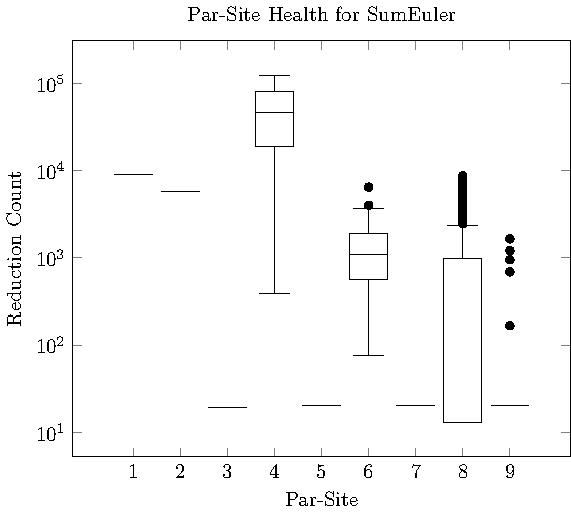
\includegraphics[width=\linewidth]{Informed/Figures/threadhealth.pdf}
\caption{Statistics on the number of reductions carried out by the threads a
\texttt{par} site sparks off}
\label{sumHist}
\end{figure}

After every execution of the program, turn off the \verb'par' site whose threads
have the lowest average reduction count. In the case of the execution statistics
displayed in Figure \ref{sumHist} we would disable \verb-par- site 2, allowing
us to avoid the overhead of all the unproductive threads it sparked off.  Then
repeat this process until switching a \verb'par' site off increases the overall
runtime of the program.

\section{Experimental Results}
\label{sec:results}

In this section we present some preliminary results and point out certain patterns
that appear in our data. 

First we introduce our benchmark programs and state the number of \verb-par-
sites that were introduced statically:

\paragraph{SumEuler}
\texttt{SumEuler} is a common parallel functional programming benchmark first introduced
with the work on the $\langle\nu, G\rangle$-Machine in 1989 \citep{vGMachine}.
The program computes the sum of mapping the euler-totient function of a list. As
this functional idiom is known to be highly parallelisable; this benchmark can
be seen as a `sanity-check' on our technique (9 \verb-par- sites).

\paragraph{Queens $+$ Queens2}
We benchmark two versions of the nQueens program. Both versions use a backtracking
algorithm to search for possible solutions. \texttt{Queens2} is a purely symbolic version
that represents the board as a list of lists (10 \verb-par- sites for \texttt{Queens} and
24 for \texttt{Queens2}).

\paragraph{SodaCount}
Solves a word search problem for a given grid of letters and a list of keywords
(15 \verb-par- sites).

\paragraph{Tak}
Small recursive numeric computation that calculates a Takeuchi number (2 \verb-par- sites).

\paragraph{Taut}
Determines whether a given predicate expression is a tautology. Attempts all assignments
of Boolean values to the variables in the given expression (15 \verb-par- sites).

\paragraph{MatMul}
List of list matrix multiplication (7 \verb-par- sites). 


\subsection*{Overheads} Whether an expression is worthwhile to evaluate in
parallel is directly tied to \emph{cost} of creating a parallel task. In order
to account for this we ran all of our experiments with the simulated overhead
cost at 3 settings. We chose the upper and lower bounds based on benchmarking parallel
functions using the Criterion library \citep{criterion}.


For each program we set our runtime system to simulate 4, 8, and 16 cores.
First, let us examine Figure \ref{table10} which displays the results of setting
the cost of task creation to 10 reductions.

% non-normalised
%    SumEuler  & 6    & 117995    & 6    & 64903      & 6    & 43279     \\
%    Queens    & 5    & 18393517  & 5    & 17427940   & 5    & 16949174  \\
%    Queens2   & 22   & 2068082   & 22   & 1045458    & 22   & 536579    \\
%    SodaCount & 3    & 808156    & 3    & 414510     & 3    & 218639    \\
%    Tak       & 1    & 11522690  & 1    & 5763328    & 1    & 2884142   \\
%    Taut      & 4    & 32790837  & 0    & 32786617   & 9    & 32785937  \\
%    MatMul    & 2    & 9377962   & 2    & 8925278    & 2    & 8699032   \\
%                       8526965
%    Clausify  & 15   & 3163940   & 15   & 1596090    & 20   & 808068    \\

\begin{figure}[ht]
\centering
  \begin{tabular}{ |l||c c|c c|c c| }
    \hline
    Program & \multicolumn{2}{c|}{4-core} & \multicolumn{2}{c|}{8-cores} & \multicolumn{2}{c|}{16-cores} \\
    \hline
            & Runs & Final     & Runs & Final      & Runs & Final \\
    \hline
    SumEuler  & 6    & 3.77      & 6    & 6.84       & 6    & 10.27     \\
    Queens    & 5    & 1.30      & 5    & 1.37       & 5    & 1.41  \\
    Queens2   & 22   & 3.91      & 22   & 7.74       & 22   & 15.07   \\
    SodaCount & 3    & 2.42      & 3    & 4.72       & 3    & 8.95    \\
    Tak       & 1    & 3.39      & 1    & 6.79       & 1    & 13.58   \\
    Taut      & 4    & 1.00      & 0    & 1.00       & 9    & 1.00  \\
    MatMul    & 2    & 1.02      & 2    & 1.07       & 2    & 1.10   \\
    \hline
  \end{tabular}
\caption{Speedups relative to sequential computation when the cost of sparking
        a task is set to 10 reductions. The number of runs corresponds to the
        number of \texttt{par} sites that have been switched off.}
\label{table10}
\end{figure}

Already there are a few interesting results. \texttt{SumEuler} performs as expected and
manages to eliminate the majority of the introduced \verb-par- sites. Recalling
Figure \ref{sumLast}, the \verb-par-s that survive the iterative improvement
are the two in the \verb-main- function and the \verb-par- in \verb-mainListS2-.
The second \verb-par- in \verb-main- and the strategy \verb-mainListS2- are,
taken together, equivalent to applying \verb-parMap euler- over the input list.
When this program is parallelised explicitly, that \verb-parMap- is usually the
only addition to the program \citep{vGMachine}. It is reassuring that our
technique converges on the same result.

The two implementations of nQueens vary drastically in their improvement, with
the more symbolic solution (\texttt{Queens2}) achieving much better results. Search
problems are known to be problematic for techniques involving strictness
analysis and usually benefit from the introduction of \emph{speculative}
parallelism \citep{hammond2000research}.

\texttt{Taut} was chosen as a benchmark program specifically because the program (as
written) did not have many opportunities for parallelism. Had our technique
managed to find any useful parallelism, we would have been surprised.

MatMul is, to us, the most surprising of the results so far. Matrix
multiplication is famously parallelisable and yet our implementation
barely breaks even! Notice that of the 7 \verb-par- sites in MatMul, only
2 are being switched off. The \verb-par- setting that the iterative
improvement converged on was not the optimal setting (we know there is at least
2 superior settings). This convergence on local maxima is something we will
discuss in \S\ref{sec:conclusion}.

While the results in Figure \ref{table10} are revealing, it could be argued that
an overhead of 10 reductions to spark off a thread is unrealistically low.
Therefore we repeat the experiments with the more realistic 100 reduction
overhead (Figure \ref{table100}) and the pessimistic case of 1000 reduction
overheads (Figure \ref{table1000}).

\begin{figure}[ht]
\centering
  \begin{tabular}{ |l||c c|c c|c c| }
    \hline
    Program & \multicolumn{2}{c|}{4-core} & \multicolumn{2}{c|}{8-cores} & \multicolumn{2}{c|}{16-cores} \\
    \hline
            & Runs & Final     & Runs & Final      & Runs & Final \\
    \hline
    SumEuler  & 6    & 3.74      & 6    & 6.81       & 6    & 10.23     \\
    Queens    & 5    & 1.29      & 5    & 1.37       & 5    & 1.41  \\
    Queens2   & 22   & 3.83      & 22   & 7.57       & 22   & 14.76  \\
    SodaCount & 3    & 2.17      & 3    & 4.23       & 3    & 8.02    \\
    Tak       & 1    & 2.36      & 1    & 4.71       & 1    & 9.42   \\
    Taut      & 9    & 1.00      & 0    & 1.00       & 9    & 1.00  \\
    MatMul    & 2    & 0.93      & 2    & 1.06       & 2    & 1.09   \\
    \hline
  \end{tabular}
\caption{Speedups relative to sequential computation when the cost of sparking
        a task is set to 100 reductions. The number of runs corresponds to the
        number of \texttt{par} sites that have been switched off.}
\label{table100}
\end{figure}

The results in Figure \ref{table100} mostly align with what we would expect to
happen if creating a parallel task incurred higher overheads: we see reduced
speedup factors and adding more cores is less likely to benefit.

The key point to take away from this set of results is that while lower speedups
are achieved, the \emph{same} \verb-par- sites are eliminated in the same
number of iterations \footnote{Except for \texttt{Taut}, which in the 4-core case now
takes 9 runs to determine that there is no parallelism in the program.}.

Now we try the same experiment again but with the less realistic 1000 reduction
overhead to create a new thread.

\begin{figure}[ht]
\centering
  \begin{tabular}{ |l||c c|c c|c c| }
    \hline
    Program & \multicolumn{2}{c|}{4-core} & \multicolumn{2}{c|}{8-cores} & \multicolumn{2}{c|}{16-cores} \\
    \hline
            & Runs & Final     & Runs & Final      & Runs & Final \\
    \hline
    SumEuler  & 6    & 3.51      & 6    & 6.40       & 6    & 9.73     \\
    Queens    & 5    & 1.26      & 5    & 1.35       & 5    & 1.40  \\
    Queens2   & 22   & 3.14      & 22   & 6.22       & 22   & 12.18  \\
    SodaCount & 12   & 1.85      & 3    & 2.08       & 1    & 1.39    \\
    Tak       & 1    & 0.57      & 1    & 1.15       & 1    & 2.32   \\
    Taut      & 12   & 1.00      & 12   & 1.00       & 7    & 1.00  \\
    MatMul    & 5    & 1.00      & 5    & 1.00       & 5    & 1.01   \\
    \hline
  \end{tabular}
\caption{Speedups relative to sequential computation when the cost of sparking
        a task is set to 1000 reductions. The number of runs corresponds to the
        number of \texttt{par} sites that have been switched off.}
\label{table1000}
\end{figure}

While the speedups are now much more moderate (when there is a speedup at all)
these results are interesting for a few reasons.

In particular, the number of cores now has a greater influence on how many
\verb-par- sites are worthwhile.  \texttt{SodaCount}, for instance, now eliminates 12 of
its 15 \verb-par- annotations in the case of 4-core execution. This fits with
our intuition that when there are fewer processing units the threads require
coarser granularity to be worthwhile. In the cases of 8 and 16-core executions
we observe that fewer \verb-par- sites are disabled, reinforcing this
intuition.

MatMul also sees a jump in the number of disabled \verb-par- sites. Sadly, this
results in even worse performance for MatMul, which should be a highly
parallelisable program.

\subsection*{Static vs. Iterative}

While the results presented in Informed/Figures \ref{table10}, \ref{table100}, and
\ref{table1000} are promising for preliminary results they are based on an
admittedly simple search heuristic. Part of our argument is that static analysis
\emph{alone} is not sufficient for good gains from implicit parallelism. Figure
\ref{fig:iters} presents a selection of results that show how the iterative
improvement affects the static placement of \verb-par- annotations.

Even in the cases where the final speedup is lower than anticipated, such as
\texttt{Queens} in Figure \ref{fig:iterQueens}, the program still benefits from the
iterative improvement. \texttt{Queens2} sees the highest payoff from iterative
improvement. Many of the \verb-par-s introduced by the static analysis
do not contribute significantly to the computation even though it is
semantically safe to introduce them. The iterative loop converges on the few
\verb-par- sites that make a significant difference.

\begin{figure}[h]
    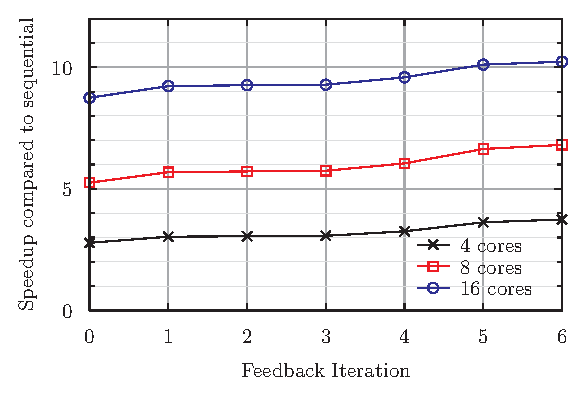
\includegraphics[scale=0.75]{Informed/Figures/IterSum.eps}
    \caption[SE]{\texttt{SumEuler} speedup}
    \label{fig:iterSum}
\end{figure}
\begin{figure}[h]
    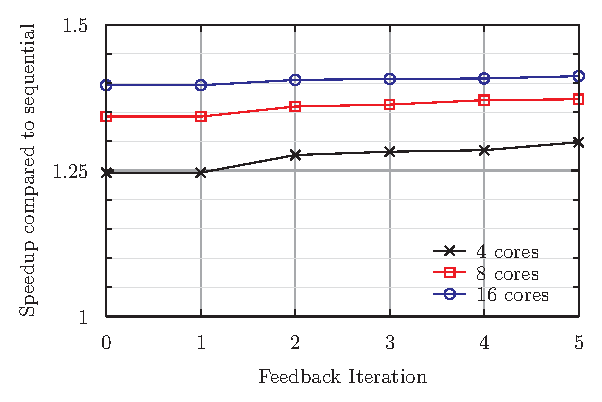
\includegraphics[scale=0.75]{Informed/Figures/IterQueens.eps}
    \caption[Q]{\texttt{Queens} speedup}
    \label{fig:iterQueens}
\end{figure}

\begin{figure}[h]
    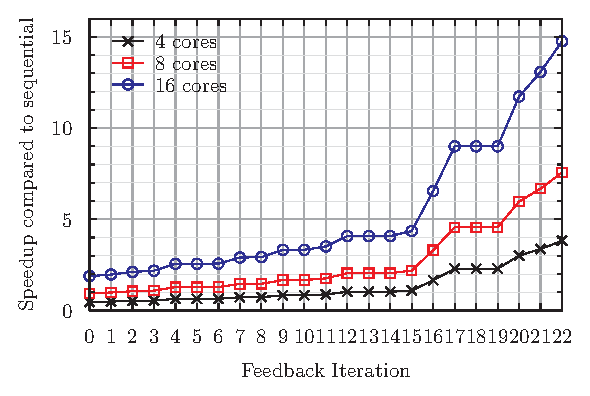
\includegraphics[scale=0.75]{Informed/Figures/IterQueens2.eps}
    \caption[Q2]{\texttt{Queens2} speedup}
    \label{fig:iterQueens2}
\end{figure}
\begin{figure}[h]
    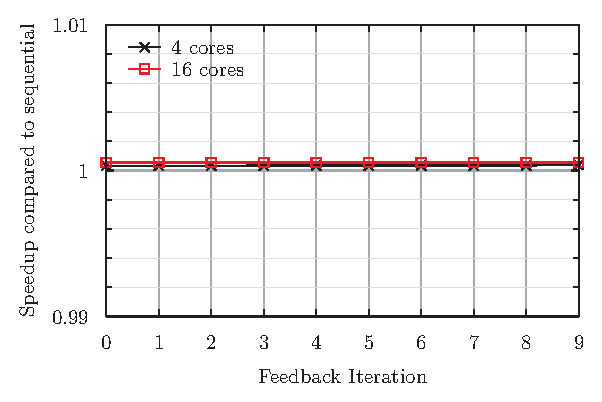
\includegraphics[scale=0.75]{Informed/Figures/IterTaut.eps}
    \caption[T]{\texttt{Taut} speedup}
    \label{fig:iterTaut}
\end{figure}


\subsection*{Comparison to GHC}

While the results above are encouraging we would like to see how the resulting
programs perform when compiled by a modern high-performance Haskell compiler.
To do this we extract the final \verb-par- settings from each program and
translate that to Haskell suitable for compilation by GHC.

For the versions parallelised by hand we use the \verb-par- placements found
in the literature \citep{vGMachine, runciman1994profiling}.

\begin{figure}[ht]
\centering
  \begin{tabular}{ |l||c c| }
    \hline
    Program & \multicolumn{2}{c|}{4-core} \\
    \hline
            & Hand   & Auto         \\
    \hline
    SumEuler  & 3.32    & 3.31      \\
    Queens    & 1.76    & 0.97      \\
    Queens2   & 2.29    & 0.61     \\
    SodaCount & 1.25    & 0.64      \\
    Tak       & 1.77    & 1.64      \\
    MatMul    & 1.75    & 0.80      \\
    \hline
  \end{tabular}
\caption{Speedups compared to the sequential program as compiled by GHC for both
         manually and automatically parallelised versions}
\label{tableGHC}
\end{figure}

As Table \ref{tableGHC} makes clear, the results are not impressive. In fact,
except for \verb-SumEuler- and \verb-Tak-, all of the parallel benchmarks
performed \emph{worse} than their sequential counterparts.

However, we feel that not all hope is lost. There are a few recurring issues in
the generated program. A common issue is that the generated strategies will not
be what forces the evaluation of a value. Take the following example as an
illustration

\begin{verbatim}
foo n = let ys = gen n n
        in par (tailStrict1 ys) (bar ys)

tailStrict1 xs = case xs of
    y:ys -> tailStrict1 ys
    []   -> ()
\end{verbatim}

In the function \verb-foo- we spark off a strategy that is meant to force the
spine of the list \verb-ys-, the catch is that GHC's \verb-par- is fast enough
for \verb-bar ys- to be what forces the evaluation of \verb-ys-. So we're
paying the overhead and reaping none of the benefits. In some programs changing
a \verb-par- like the one found in \verb-foo- to a \verb-seq- is enough to solve the
issue and make the parallel version competitive with the manually parallelised version.



\section{Conclusions}
\label{sec:conclusion}


We hope we have motivated the key design choices and ideas behind our compiler:
utilising defunctionalisation in \S\ref{sec:defunct}, and the use of
projections over other strictness analysis methods in \S\ref{sec:strictness}.
Moreover, that we have shown that there is a natural correspondence between
projections and strategies \S\ref{sec:proAndStrat} that allows us to generate
parallel strategies from the results of our strictness analysis.

While projection-based strictness analysis does provide a useful foundation for
the introduction of parallelism, the results in \S\ref{sec:results} show that
static analysis alone does not provide the desired speedups. Additionally,
Table \ref{tableGHC} shows that determining \verb-par--site health by reduction
count alone is too naive. Thread collisions that may not happen on a simulated
system are able to significantly hamper parallel performance and should be
taken into account.

\subsection{Related Work}

\subsection*{Hinze's Work on Projections} 

Much of the early work on strictness
analysis as a means to achieve implicit parallelism focused on the abstract
interpretation approach because the work on projections had not been fully
developed when implicit parallelism was a more active research area. In
particular, the work on the ``Automatic Parallelization of Lazy Functional
Programs'' \citep{hogen1992automatic} only used two and four-point domains (as
described in \citep{wadler1987strictness}) in their strictness analysis. This
limits the ability of the compiler to determine the neededness of more complex
structures.

Hinze's work on projection-based strictness analysis came after work on implicit
parallelism fell out of favour \citep{hinze1995projection, hammond2000research}. To
our knowledge we are the first to apply this work to the implicit parallelism.

\subsection*{Blind Search}

By representing a program's \verb-par- settings as a bit string we can
experiment with standard search techniques. Many algorithms can optimise a
function using only a fitness function that takes a bitstring as an input. In
our case, the compiler would set the \verb-par- switches according to the
bitstring and use the wall-clock time as a fitness function.  We explored two
such algorithms in an earlier paper showing that even simple search algorithms,
such as hill-climbing, can achieve promising results \citep{ssbse}. The downside
to these techniques is that they require a large number of iterations to
converge. The technique presented here allows us to get similar results in
linear (in the length of the bitstring) time.

As we attempt to scale our technique to larger programs it is likely that blind
search technique will run into the combinatorial explosion inherent in
bitstring-based search techniques.


\subsection*{Implicit Parallelism}

As the quote from the start of the paper alludes to, there are few modern
attempts at implicit parallelism for lazy functional languages.
One significant exception to this is the work undertaken in 2007 by Harris and
Singh \citep{feedbackImplicit}. The results were mostly positive
(in that most benchmarks saw an improvement in performance) but were not to the degree
desired. Since this research was published we have seen no other attempt in
this line of research within the lazy functional programming community.

The approach presented here can be seen as the inverse
of the approach by Harris et al. \citep{feedbackImplicit} where the compiler
starts with \emph{no} parallelism and the iterative feedback seeks to add
parallel evaluation.

The work in \citep{feedbackImplicit} attempted to use runtime profile data to introduce
parallel annotations into the program based on heap allocations. In short, when viewing
the parallel execution of a program as a tree, their method seeks to expand the tree
based on previous executions of the program. Our goal is to develop a system
that begins with a program that perhaps has \emph{too much} parallelism and
uses runtime data to prune the execution tree. We have implemented a few mechanisms
to make this possible.

\subsection*{Semi-implicit Parallelism}
Research into semi-implicit parallelism for lazy functional languages is still
an active research area. The work on Repa frees the programmer from worrying
about parallelism in array computations by hiding the parallel details behind an
API \citep{repa}. GPGPU parallelism is also well studied and has resulted in the
popular high-performance Haskell library Accelerate \citep{accelerate}.

\subsection{Future Work}

\paragraph{\texttt{par} Health} Other forms of penalties need to be introduced.
Blocking other threads, being blocked for extended periods of time, creating
too many parallel threads (or not enough) could all be measures that incur a
penalty. One simple but effective metric would be to penalise \verb-par- sites
that spark strategies that are not the first to evaluate their arguments. When
another thread forces the evaluation of a structure before the strategy that
was meant to, we lose the benefit of parallel strategies. These penalties would
factor in to the \verb-par- site's `health' and determine which site should be
disabled before the next iteration.

\paragraph{Specialisation}

One area that we expect to explore is the use of other forms of specialisation.
Defunctionalisation specialises higher-order functions to first-order ones.
Other possibilities include specialising polymorphic functions into their
monomorphic versions and specialising functions based on their call-depth.
Specialising based on call-depth is a common technique in hand written programs.
Automating the process could lead to significant improvements in recursive
numeric programs (such as \texttt{Tak}).

\paragraph{Path Analysis} One goal of our work is to determine when it is
appropriate to use parallelism in a strategy.  Currently, we spark constructor
fields in a left-to-right order but we believe that performing a path analysis
would aid in this task \citep{bloss1994path}. Path analysis can also help reduce
the chances of thread collisions statically. By determining which expression
will force a value first we can avoid one of the central shortcomings of the
approach outlined in this paper.
